\section{Background}
\label{sec:background}

Radio searches for technosignatures began at centimetre wavelengths and
have largely stayed there. The first targeted experiments
\citep{CocconiMorrison1959,Drake1960}, the programmes reviewed by
\citet{Tarter2001} and Project Phoenix \citep{Backus2002} all worked
below a few gigahertz. The modern generation divides into targeted and
commensal surveys at centimetre and metre wavelengths
\citep{Zhang2020,Czech2021,FAST3IATLAS2025,LOFARdualsite2023,Choza2024},
several of them riding back-ends built for other science
\citep{Morrison2023}, with wide-field low-frequency coverage from the MWA
\citep{Tremblay2024}
and single-dish C- and K-band work at 6 and 18\,GHz with the Sardinia
Radio Telescope \citep{SRT2025}. Machine-learning interference rejection
is now central to that effort
\citep{Ma2023,GLOBULAR2025,AnomalyParkesGBT2025}. The
classical threshold search used here lacks that capability, and instead
uses a spatial test on the star against control positions in the same
field, which a single dish cannot make. A narrowband search also reaches
only one class of signal: broadband planetary-scale leakage
\citep{BRaTs2026} is outside it by construction.

Above about 30\,GHz the record is nearly empty, and that is what makes
this frequency range new. ALMA observes in Bands~3 to~10, spanning
roughly 84 to 950\,GHz; of those eight bands, one has been searched for
technosignatures. For continuity with the centimetre literature we note
one familiar power scale: the Arecibo planetary radar radiated
$\AreciboW$\,W at \ArecGHz\,GHz
\citep{EarthDetectingEarth2025}. It carries no transmitter
model into the millimetre band, where an aperture of that diameter is not
realisable, so the illustrative benchmark of \S\ref{sec:excludes} is
instead a dish of \BenchDiam\,m. Neither is a privileged scale; the limits
of this paper are stated as EIRP and need no transmitter model.

\citet{Mason2025} is the only prior millimetre search and the only
comparable archival one. They searched Band~3 windows toward
\MasonNStar{} Gaia~DR3 stars lying in the fields of \MasonNCal{} ALMA
calibrators, observed for other science and so usable for free. Their
nearest target is at \MasonNearKpc\,kpc, where a $5\sigma$ flux threshold
corresponds to EIRP$_{\rm min}>{}$\MasonNearEirp\,W. That target lies
\MasonDistRatioFar$\times$ further away than the most distant star searched
here for a carrier and \MasonDistRatioNear$\times$ further than the nearest
of those: the two
samples differ by \MasonDistOrdLo--\MasonDistOrdHi{} orders of magnitude in
distance, and at a fixed received flux by the square of that, which is
\MasonEirpOrdLo--\MasonEirpOrdHi{} orders in minimum detectable EIRP. An EIRP
ratio between the two surveys would therefore be almost entirely the $d^{2}$
term. The quantity
that does not depend on distance is the minimum detectable \emph{received}
flux, $F_{\rm min}=S_{\rm min}\,\delta\nu$. It must be quoted at a matched
channel width, because $S_{\rm min}$ falls as $\delta\nu^{-1/2}$ while
$F_{\rm min}$ rises as $\delta\nu^{1/2}$. Mason
et~al.\ reach \MasonFluxLo--\MasonFluxHi\,W\,m$^{-2}$ across their four
fields, on a \MasonChanKHz\,kHz channel at a bare $5\sigma$ flux
threshold. On
that same channel width and the same threshold convention, the
fine-channel windows searched here reach \FluxMatchBest\,W\,m$^{-2}$ at
best, a factor \FluxBestRatio{} deeper, and \FluxMatchMed\,W\,m$^{-2}$ at
the median, a factor \FluxMedRatio{} shallower. The two experiments are
therefore comparable in depth and differ in what they cover: distant stars
in four calibrator fields, against \NSysClassA{} stellar systems within
40\,pc searched for a drifting carrier, over a frequency range reaching
about nine times higher. They also
identified the obstacles that shape the present method: drift rates scale
with frequency, smearing erodes sensitivity unless drift is searched for,
and the dense forest of molecular lines raises the confusion background.
Every window reported here was re-reduced and re-searched from the raw
archive data with the pipeline of \S\ref{sec:method}, so for any star in
common the numbers to cite are this paper's.

Figure~\ref{fig:context}(a) places this survey among published searches,
in minimum detectable EIRP against distance. The vertical axis is
physically commensurable: for a carrier narrower than every programme's
channel, the minimum detectable EIRP is a total radiated power and not a
spectral power density, so the same quantity is plotted for each
programme. What differs is the convention, so both are drawn. Every
published limit shown is a nominal $5\sigma$ threshold at which recovery
is not stated, and this survey's filled symbols are the same thing
measured the same way; the open symbols above them are
$\mathrm{EIRP}_{90}$, a 90 per cent recovery through the complete
automated selection, which is the stricter statement and the one every
limit in this paper is quoted on. Any EIRP advantage toward the nearest
systems is a $d^{2}$ effect and not an instrumental one. Panel~(b) shows the other axis that matters.
Archived correlator channels here span \SzChanDexSurvey{} orders of
magnitude in width, from \SzChanFinestKHz\,kHz to
\SzChanWidestMHz\,MHz, and all of them are far coarser than a dedicated
narrowband backend, whose \SzChanLitHz\,Hz channels open the full seven
orders only when they are set beside ours. The distinctive feature of this survey is therefore its
frequency regime and its channelisation, not its depth. It also samples far
fewer systems and far fewer
epochs than a dedicated search, and complements those programmes rather
than deepening them.

\begin{figure}
\centering
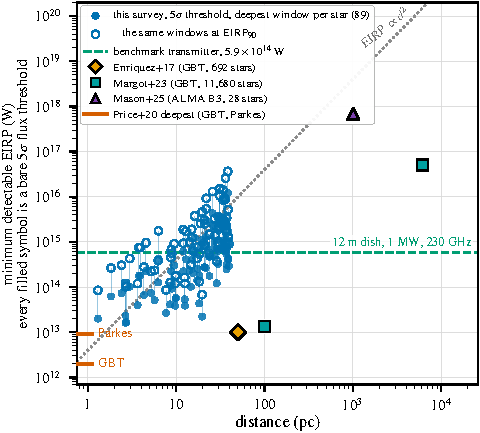
\includegraphics[width=\columnwidth]{figures/eirp_context_a.pdf}\\
{\footnotesize (a)}\\[4pt]
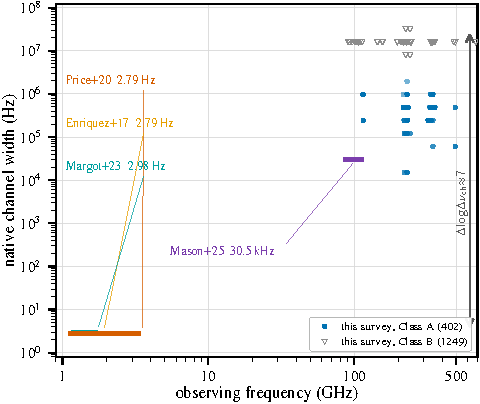
\includegraphics[width=\columnwidth]{figures/eirp_context_b.pdf}\\
{\footnotesize (b)}
\caption{Where this survey sits among published radio technosignature
searches. \textbf{(a)} Minimum detectable EIRP against distance. Blue,
this survey, the deepest window per star: \emph{filled}, that window's bare
$5\sigma$ threshold, which is the quantity the other programmes quote;
\emph{open}, the same window at $\mathrm{EIRP}_{90}$, joined to its own
filled symbol. Orange, \citet{Enriquez2017}; aqua, \citet{Margot2023};
violet, \citet{Mason2025}; left-edge ticks, \citet{Price2020}, all at their
own $5\sigma$ thresholds. Grey dotted, EIRP $\propto d^{2}$ at constant
received flux; green dashed, the illustrative \BenchDiam\,m
benchmark transmitter of \S\ref{sec:excludes}. The ordinates are
commensurable as total powers for a sub-channel carrier, and the filled
symbols make the comparison on one convention; the gap to the open symbol
is what completeness costs.
\textbf{(b)} Native channel width against observing frequency for every
searched window (filled, Class~A; open, Class~B), with the
comparison programmes as horizontal segments. This survey's own widths span
\SzChanDexSurvey{} orders of magnitude; the
$\Delta\log\Delta\nu_{\rm ch}\approx7$ annotation marks the span that
opens once the comparison programmes' channels are set beside them: the
channelisation, not the plotted power, is what differs most between
programmes.}
\label{fig:context}
\end{figure}

A non-detection becomes a quantitative statement only through a stated
search volume. \citet{Wright2018} formalised that volume, and
\citet{Margot2023} its conversion into an upper bound on the fraction of
stars hosting a transmitter; \citet{EarthDetectingEarth2025} asked where
Earth's own technosignatures would be detectable. Such a bound is valid
only if the sample represents the population it is meant to describe.
This sample was assembled by other observers for other purposes, so it
does not, and \S\ref{sec:sample} states what it is instead.

%% Glenn's instruction, verbatim: the appendices are deliberately detailed and the
%% paper says so, so that a reader meets them as intended rather than as padding.
Because of the very specific and detailed statistical nature of this study, we have
extended the paper to include several very detailed Appendices that rigorously
explain the methodology involved.

%% Housekeeping, v4.12: the three standing REQUESTs that lived here are now
%% moot. app_D, app_E and app_F have been deleted, so fig:contextapp and the
%% three unlettered \ref{fig:context} citations they carried are gone with
%% them; 05_results.tex writes Fig.~\ref{fig:context}(a) in full.
%% STILL OPEN, and queued for the sensitivity owner rather than repeated
%% here: referee 2's figure point 1 asks that panel (a) plot this survey's
%% 5 sigma EIRP_trig as the filled symbol, for a like-for-like comparison
%% with the other programmes' bare thresholds, and EIRP_90 as a second open
%% symbol on the same points. The caption above already concedes that the
%% conventions differ, which is the concession the referee is declining to
%% accept; it must become two symbols, not a sentence.
%% The Mason matched-received-flux comparison is made here and nowhere else;
%% \S6 cites this section for it. The benchmark is evaluated once, in
%% \S\ref{sec:excludes}, and is labelled illustrative in both places it is
%% named.
